% =============================================================================
%  showcase.tex - a one-page overview of LaTeX Studio.
%
%  Doubles as a demo document: it deliberately exercises the features the app
%  has to get right (TikZ, tcolorbox, tables, maths, colour, hyperlinks) so that
%  compiling it is itself a test of the compiler.
%
%  Compile with: pdflatex (no shell-escape needed).
% =============================================================================
\documentclass[a4paper,10pt]{article}

\usepackage[margin=1.1cm]{geometry}
\usepackage[T1]{fontenc}
\usepackage{lmodern}
\usepackage{xcolor}
\usepackage{tikz}
\usepackage[most]{tcolorbox}
\usepackage{booktabs}
\usepackage{enumitem}
\usepackage{amsmath}
\usepackage{fontawesome5}
\usepackage[hidelinks]{hyperref}

\usetikzlibrary{positioning, arrows.meta}

% ─── Brand palette (matches the app's own dark UI) ───────────────────────────
\definecolor{ink}{HTML}{0D1117}        % near-black background
\definecolor{surface}{HTML}{161B22}    % panel background
\definecolor{accent}{HTML}{22C55E}     % primary green
\definecolor{accentlite}{HTML}{4ADE80} % lighter green
\definecolor{muted}{HTML}{8B949E}      % secondary text
\definecolor{paper}{HTML}{F6F8FA}

\pagestyle{empty}
\setlength{\parindent}{0pt}

% A compact stat tile: \stat{number}{label}
\newcommand{\stat}[2]{%
  \begin{tcolorbox}[colback=surface, colframe=accent, boxrule=0.4pt,
                    arc=2pt, left=3pt, right=3pt, top=3pt, bottom=3pt,
                    width=\linewidth, halign=center]
    {\color{accentlite}\Large\bfseries #1}\\[-1pt]
    {\color{muted}\scriptsize #2}
  \end{tcolorbox}}

% A feature panel: \feature{icon}{title}{body}
\newcommand{\feature}[3]{%
  \begin{tcolorbox}[colback=paper, colframe=accent!55!white, boxrule=0.6pt,
                    arc=3pt, left=6pt, right=6pt, top=4pt, bottom=4pt,
                    width=\linewidth]
    {\color{accent}#1}~{\bfseries #2}\\[1pt]
    {\footnotesize #3}
  \end{tcolorbox}}

\begin{document}

% ═══════════════════════════ HEADER BAND ═══════════════════════════════════
\begin{tcolorbox}[colback=ink, colframe=ink, arc=4pt,
                  left=14pt, right=14pt, top=10pt, bottom=10pt]
  \begin{minipage}[c]{0.60\linewidth}
    {\color{white}\Huge\bfseries LaTeX\,\color{accentlite}Studio}\par\vspace{4pt}
    {\color{muted}\normalsize Write and compile LaTeX in your browser,
     on your own machine.}
  \end{minipage}\hfill
  \begin{minipage}[c]{0.36\linewidth}\raggedleft
    {\color{accentlite}\footnotesize\faGithub~\texttt{github.com/AhmedOuf19/LatexOS}}\par\vspace{3pt}
    {\color{muted}\footnotesize v1.2.0 \; $\cdot$ \; MIT licence \; $\cdot$ \; Windows}
  \end{minipage}
\end{tcolorbox}

\vspace{10pt}

% ═══════════════════════════ STAT ROW ══════════════════════════════════════
\noindent
\begin{minipage}[t]{0.235\linewidth}\stat{110}{automated tests}\end{minipage}\hfill
\begin{minipage}[t]{0.235\linewidth}\stat{100\,\%}{documented API}\end{minipage}\hfill
\begin{minipage}[t]{0.235\linewidth}\stat{3}{TeX engines}\end{minipage}\hfill
\begin{minipage}[t]{0.235\linewidth}\stat{0}{cloud uploads}\end{minipage}

\vspace{16pt}

% ═══════════════════════════ TWO COLUMNS ═══════════════════════════════════
\noindent
\begin{minipage}[t]{0.49\linewidth}

  % \par + \vspace rather than \\ : a forced break after a short heading
  % stretches it to the full column width and logs an underfull hbox.
  {\color{accent}\large\bfseries What it does}\par\vspace{4pt}

  \feature{\faBolt}{Compiles while you type}
    {pdfLaTeX, XeLaTeX and LuaLaTeX, with bibliographies, multi-file projects
     and custom classes handled automatically.}

  \vspace{3pt}
  \feature{\faMagic}{Installs packages for you}
    {Use \texttt{\textbackslash usepackage\{tikz\}} without installing anything:
     a missing package is fetched on demand, mid-compile.}

  \vspace{3pt}
  \feature{\faExclamationTriangle}{Explains the errors}
    {The log is parsed into errors and warnings with file and line numbers,
     plus plain-language hints for the cryptic ones.}

  \vspace{3pt}
  \feature{\faBoxOpen}{Portable by design}
    {Python, LaTeX, the editor and the fonts all install \emph{into the project
     folder}. No admin rights. Delete the folder to uninstall.}

\end{minipage}\hfill
\begin{minipage}[t]{0.49\linewidth}

  {\color{accent}\large\bfseries How it works}\par\vspace{6pt}

  \centering
  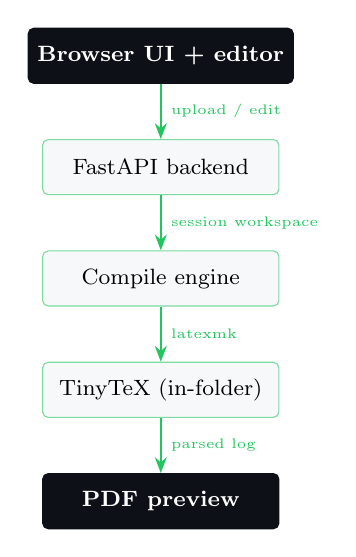
\begin{tikzpicture}[
      node distance=7mm,
      box/.style={draw=accent!60!white, fill=paper, rounded corners=2pt,
                  minimum width=30mm, minimum height=7mm, font=\footnotesize},
      dark/.style={draw=ink, fill=ink, text=white, rounded corners=2pt,
                   minimum width=30mm, minimum height=7mm, font=\footnotesize\bfseries},
      arrow/.style={-{Stealth[length=2mm]}, accent, thick}]
    \node[dark]              (ui)   {Browser UI + editor};
    \node[box, below=of ui]  (api)  {FastAPI backend};
    \node[box, below=of api] (comp) {Compile engine};
    \node[box, below=of comp](tex)  {TinyTeX (in-folder)};
    \node[dark, below=of tex](pdf)  {PDF preview};
    \draw[arrow] (ui)   -- node[right, font=\tiny\color{muted}] {upload / edit} (api);
    \draw[arrow] (api)  -- node[right, font=\tiny\color{muted}] {session workspace} (comp);
    \draw[arrow] (comp) -- node[right, font=\tiny\color{muted}] {latexmk} (tex);
    \draw[arrow] (tex)  -- node[right, font=\tiny\color{muted}] {parsed log} (pdf);
  \end{tikzpicture}

  \vspace{6pt}
  \raggedright
  {\color{accent}\large\bfseries Safe by default}\\[3pt]
  {\footnotesize
  \begin{tabular}{@{}ll@{}}
    \toprule
    \textbf{Guard} & \textbf{Default} \\
    \midrule
    Shell escape (\texttt{\textbackslash write18})  & off, opt-in \\
    File access                                     & workspace only \\
    Network binding                                 & \texttt{127.0.0.1} \\
    Uploads                                         & size + type capped \\
    \bottomrule
  \end{tabular}}

\end{minipage}

\vspace{23pt}

% ═══════════════════════════ GET STARTED ═══════════════════════════════════
{\color{accent}\large\bfseries Get started in three steps}\par\vspace{6pt}

\noindent
\begin{minipage}[t]{0.32\linewidth}
  \begin{tcolorbox}[colback=paper, colframe=accent!55!white, boxrule=0.6pt,
                    arc=3pt, left=7pt, right=7pt, top=5pt, bottom=5pt,
                    height=2.45cm, valign=center]
    {\color{accent}\bfseries 1 \; Download}\par\vspace{2pt}
    {\footnotesize Clone the repository, or grab the ZIP from the
     latest release.}
  \end{tcolorbox}
\end{minipage}\hfill
\begin{minipage}[t]{0.32\linewidth}
  \begin{tcolorbox}[colback=paper, colframe=accent!55!white, boxrule=0.6pt,
                    arc=3pt, left=7pt, right=7pt, top=5pt, bottom=5pt,
                    height=2.45cm, valign=center]
    {\color{accent}\bfseries 2 \; \texttt{install.bat}}\par\vspace{2pt}
    {\footnotesize One click. Fetches Python, TinyTeX and the editor into the
     folder. No admin rights.}
  \end{tcolorbox}
\end{minipage}\hfill
\begin{minipage}[t]{0.32\linewidth}
  \begin{tcolorbox}[colback=ink, colframe=accent, boxrule=0.6pt,
                    arc=3pt, left=7pt, right=7pt, top=5pt, bottom=5pt,
                    height=2.45cm, valign=center]
    {\color{accentlite}\bfseries 3 \; Launch}\par\vspace{2pt}
    {\color{white}\footnotesize Your browser opens. Drop in a project and
     press \textbf{Compile}.}
  \end{tcolorbox}
\end{minipage}

\vspace{22pt}

% ═══════════════════════════ PROOF IT TYPESETS ═════════════════════════════
\begin{tcolorbox}[colback=paper, colframe=accent!55!white, boxrule=0.6pt,
                  arc=3pt, left=10pt, right=10pt, top=7pt, bottom=7pt]
  \begin{center}
    {\color{accent}\bfseries\faCheckCircle~This page was rendered by the app itself.}\par\vspace{2pt}
    {\footnotesize Every element above --- the diagram, the panels, the table ---
     and the mathematics below, compiled in one click.}
  \end{center}
  \vspace{2pt}
  \[
    \mathcal{L}\{f\}(s)=\int_{0}^{\infty} f(t)\,e^{-st}\,\mathrm{d}t
    \qquad
    e^{i\pi}+1=0
    \qquad
    \sum_{n=1}^{\infty}\frac{1}{n^{2}}=\frac{\pi^{2}}{6}
  \]
\end{tcolorbox}

\vfill

\begin{center}
  {\color{muted}\footnotesize
  Built with FastAPI, Monaco Editor and TinyTeX \; $\cdot$ \;
  Open source, contributions welcome \; $\cdot$ \;
  \faGithub~\texttt{github.com/AhmedOuf19/LatexOS}}
\end{center}

\end{document}
